\documentclass{article}
\usepackage[T1]{fontenc}
\usepackage{lmodern}
\usepackage{graphicx}
\usepackage{amsmath,amssymb}
\usepackage[a4paper,margin=2cm]{geometry}
\usepackage[absolute,overlay]{textpos}
\setlength{\TPHorizModule}{1mm}
\setlength{\TPVertModule}{1mm}
\usepackage[indonesian]{babel}
\usepackage{hyperref}
\setlength{\emergencystretch}{2em}
% unit: Halaman 32

\begin{document}

% === Halaman 32 (llm) ===

\vspace{172.26mm}

Sumber: William Stalling, Cryptography and Network Security
Overview & Chapter 1

\vspace{60mm}

\textbf{Passive Attack : Traffic Analysis}

% deskripsi: Diagram yang mengilustrasikan analisis lalu lintas (traffic analysis) sebagai serangan pasif, menampilkan Bob dan Alice yang berkomunikasi melalui Internet atau fasilitas komunikasi lainnya, sementara penyerang bernama Darth mengamati pola lalu lintas data tersebut.
% bbox normalisasi: [0.1400, 0.1400, 0.7800, 0.7200]
\begin{textblock*}{134.40mm}(29.40mm,41.58mm)
\noindent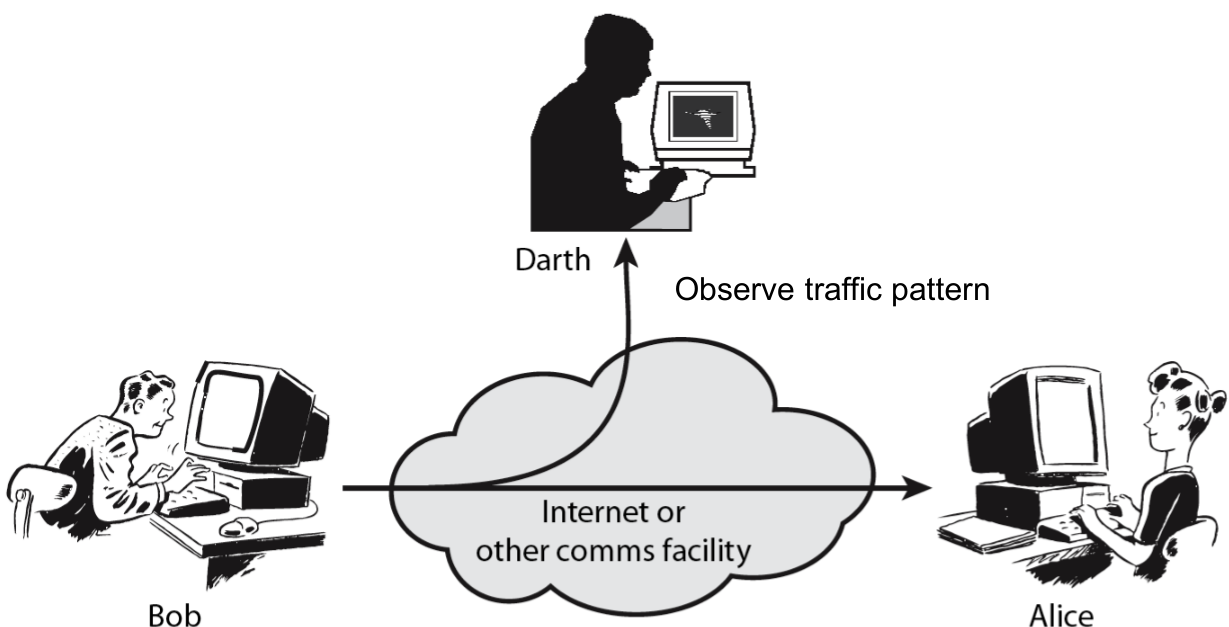
\includegraphics[width=134.40mm,height=172.26mm]{../../images/llm/page_032_img_01.png}%
\end{textblock*}

\end{document}
